\section{2D Morphogenesis With Coordinate Inputs}
\label{sec:morphXY}
Adding environmental information to the CA may make it possible to solve a task that is difficult with only the neighborhood information.
The morphogenesis task makes for a nice test case.
For this experiment, the cellular model is extended to include coordinate information, as described in Section \ref{sec:input_extensions}.
The "Border" and "Nordic" patterns (Figure \ref{fig:patterns}) are targeted in separate experiments.
The "Border" morphogenesis in the previous experiment did not work very well, so it makes for a good comparison.
The "Nordic" pattern is also difficult to generate with the cellular model (TODO because), so it was not attempted in the previous experiment,
but is attempted now.

The quiescent rule is still in place: a cell may not change state if all the neighbors are quiescent, even if the information from the coordinates is available to inform a decision.
The coordinate information is meant to be used in conjunction with the neighborhood information, not to replace it.
If this was not the case, evolution could come up with a CPPN where all the neighborhood inputs were disconnected from the output,
and a static pattern was produced in one time step, like in Figure \ref{fig:cppn}.
That is not a result that we are interested in.

\subsection{Results}

\begin{figure}
\centering
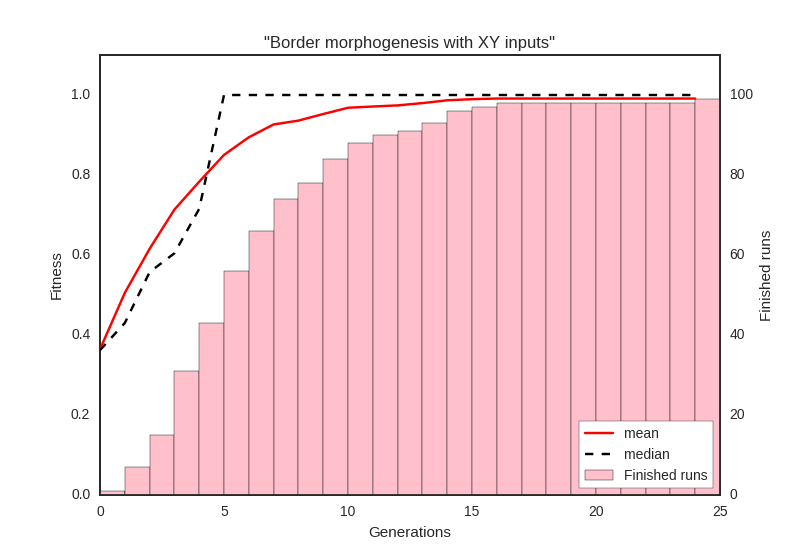
\includegraphics[width=\textwidth, keepaspectratio]{fig/generate_border_extended_results}
\caption{
    TODO
    One trial had yet to succeed when the experiment was stopped at 100 generations.
}
\label{fig:generate_border_extended_result}
\end{figure}


\begin{figure}
\centering
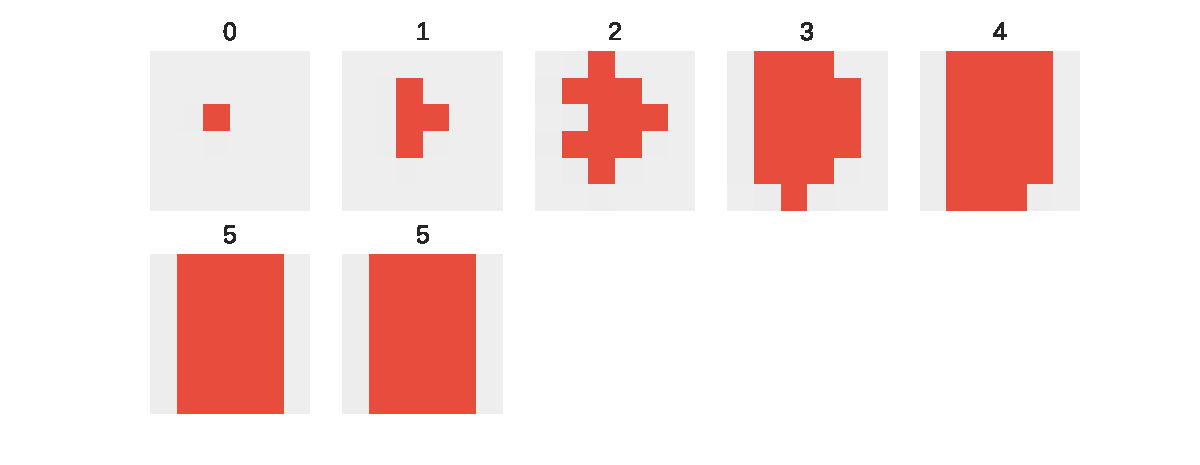
\includegraphics[width=\textwidth, keepaspectratio]{fig/result_figs/border_point_5}
\caption{
    TODO
}
\label{fig:border_point_5}
\end{figure}

TODO
